\documentclass[11pt,a4paper]{article}

\usepackage[utf8]{inputenc}
\usepackage[T1]{fontenc}
\usepackage{lmodern}
\usepackage[english]{babel}
\usepackage[a4paper,margin=22mm]{geometry}
\usepackage{microtype}
\usepackage{graphicx}
\usepackage{xcolor}
\usepackage{booktabs}
\usepackage{tabularx}
\usepackage{array}
\usepackage{enumitem}
\usepackage{caption}
\usepackage{float}
\usepackage{fancyhdr}
\usepackage{titlesec}
\usepackage{hyperref}

\definecolor{navy}{HTML}{102A43}
\definecolor{blue}{HTML}{1F5F99}
\definecolor{teal}{HTML}{0F8B74}
\definecolor{muted}{HTML}{586B7C}
\definecolor{soft}{HTML}{F3F7FA}
\definecolor{line}{HTML}{D7E1EA}
\definecolor{finding}{HTML}{B83A2F}

\hypersetup{
  colorlinks=true,
  linkcolor=navy,
  urlcolor=blue,
  pdftitle={UVM Verification of a P4 Adder and a Windowed Register File},
  pdfauthor={Erfan Taheri}
}

\titleformat{\section}{\Large\bfseries\color{navy}}{\thesection}{0.65em}{}[\color{line}\titlerule]
\titleformat{\subsection}{\large\bfseries\color{navy}}{\thesubsection}{0.55em}{}
\titleformat{\subsubsection}{\normalsize\bfseries\color{navy}}{\thesubsubsection}{0.5em}{}
\setlist[itemize]{leftmargin=5mm,itemsep=2pt,topsep=4pt}
\setlist[enumerate]{leftmargin=6mm,itemsep=2pt,topsep=4pt}
\captionsetup{font=small,labelfont=bf,textfont=it}
\renewcommand{\arraystretch}{1.18}
\newcolumntype{Y}{>{\raggedright\arraybackslash}X}
\newcommand{\code}[1]{\texttt{#1}}

\pagestyle{fancy}
\setlength{\headheight}{22pt}
\fancyhf{}
\fancyhead[L]{\small\color{muted}UVM verification portfolio}
\fancyhead[R]{\small\color{muted}Erfan Taheri}
\fancyfoot[C]{\small\color{muted}\thepage}
\renewcommand{\headrulewidth}{0.3pt}
\renewcommand{\headrule}{\hbox to\headwidth{\color{line}\leaders\hrule height \headrulewidth\hfill}}

\begin{document}

\begin{titlepage}
  \color{navy}
  \vspace*{28mm}
  {\small\bfseries\color{teal}\MakeUppercase{Public technical report}\par}
  \vspace{16mm}
  {\Huge\bfseries UVM Verification of a P4 Adder and a Windowed Register File\par}
  \vspace{8mm}
  {\Large\color{muted}Coverage-driven verification at RTL and after synthesis\par}
  \vspace{18mm}
  \noindent{\color{teal}\rule{\textwidth}{1.2pt}}
  \vfill
  {\large\bfseries Erfan Taheri\par}
  \vspace{2mm}
  {\color{muted}SoC Verification Strategies\par}
\end{titlepage}

\pagenumbering{roman}
\tableofcontents
\clearpage
\pagenumbering{arabic}

\section{Introduction}

This report presents two Universal Verification Methodology (UVM) environments developed for a registered 32-bit P4 adder and a 64-bit windowed register file. The common objective was to create self-checking, coverage-driven environments in which an independent model decides correctness and coverage reports guide closure. The two environments share an agent, monitor, scoreboard, sequence layering, and functional coverage, but their timing models and verification targets are different.

\begin{table}[H]
\centering
\caption{RTL scope and verification focus.}
\begin{tabularx}{\textwidth}{@{}p{0.22\textwidth}YY@{}}
\toprule
\textbf{Block} & \textbf{RTL summary} & \textbf{Verification focus} \\
\midrule
P4 adder & Registered 32-bit sparse-tree carry-select adder divided into eight 4-bit carry blocks, with a fixed two-cycle input-to-output latency. & Pipeline alignment, arithmetic correctness, block propagate and generate behavior, full-width carry ripple, prefix-tree expression terms, and reset behavior. \\
Windowed register file & Eight overlapping windows, eight fixed global registers, 136 physical 64-bit registers, and a window-management state machine controlled by \code{CALL} and \code{RET}. & Address translation, adjacent-window overlap, registered reads, CWP/SWP transitions, save/restore counters, spill/fill boundaries, fixed-map globals, and RAL access. \\
\bottomrule
\end{tabularx}
\end{table}

The adder verification concentrates on a pipelined arithmetic datapath and the internal conditions that activate its carry tree. The register-file verification is stateful and cycle accurate: each monitored transaction represents one clock, and the reference model advances the physical array and window-management state in lockstep with the RTL.

\clearpage
\section{P4 adder verification}

\subsection{Verification goal and checklist}

The verification goal is to prove that the registered adder returns the correct 33-bit arithmetic result at the specified latency and that stimulus exercises the carry architecture, not only representative operand values.

\begin{table}[H]
\centering
\caption{P4 specification checklist.}
\begin{tabularx}{0.96\textwidth}{@{}p{0.28\textwidth}Y@{}}
\toprule
\textbf{Requirement} & \textbf{Acceptance criterion} \\
\midrule
Arithmetic result & For every checked transaction, \(\{C_{out},S\}=A+B+C_{in}\). \\
Pipeline timing & The result observed at cycle \(T+2\) is paired with the operands accepted at cycle \(T\). \\
Reset & Registered datapath state clears, and the monitor discards transactions invalidated by reset. \\
Carry architecture & Every 4-bit block exercises propagate, generate, incoming-carry, and actual ripple behavior. \\
Critical cases & Arithmetic corners, carry input/output, full-width propagation, and non-masking prefix-tree terms are exercised. \\
Implementation reuse & The same checker and functional-coverage model run on the mapped netlist, and the timing constraint is met. \\
\bottomrule
\end{tabularx}
\end{table}

\subsection{RTL behavior and verification focus}

The DUT combines a sparse parallel-prefix carry generator with carry-select sum blocks. The 32-bit datapath is partitioned into eight 4-bit blocks. Input and output registers create a fixed two-cycle latency, so the monitor must associate each observed result with the operands accepted two cycles earlier.

The scoreboard computes the expected 33-bit result independently as
\[
  \{C_{out},S\}=A+B+C_{in}.
\]
The arithmetic operator does not reproduce the RTL carry tree. A defect in the tree therefore cannot be copied into the expected result. Four-state comparison is used so that an undefined DUT output is treated as a mismatch.

\begin{figure}[H]
  \centering
  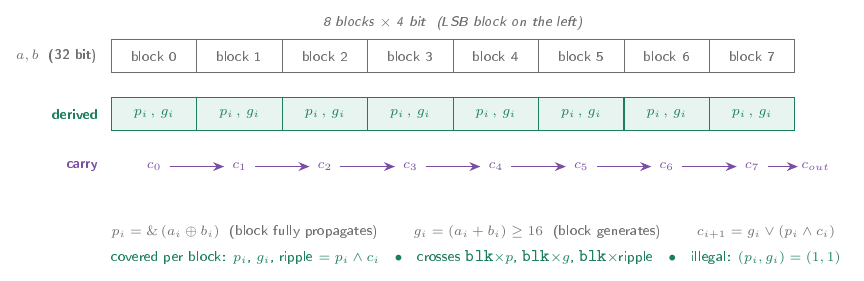
\includegraphics[width=0.99\textwidth]{../p4-adder/figures/coverage-model.png}
  \caption{P4 block structure and the architecture-aware quantities derived for coverage.}
\end{figure}

\subsection{UVM environment and timing model}

The sequencer and driver apply one addition per transaction through a clocking-block interface. The monitor maintains a two-entry pipeline of operands and publishes only complete \((A,B,C_{in},S,C_{out})\) transactions. The scoreboard therefore receives aligned data and remains independent of the DUT latency. The same monitored stream feeds the functional-coverage collector.

\begin{figure}[H]
  \centering
  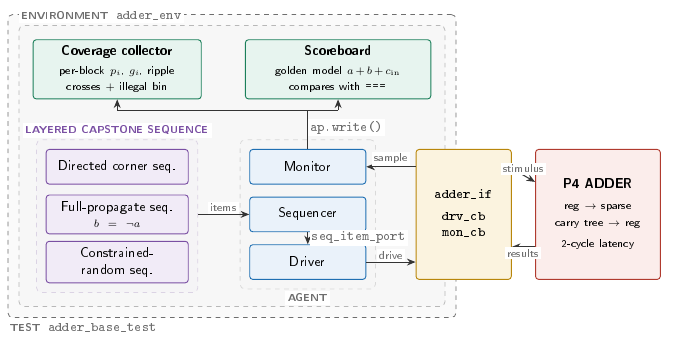
\includegraphics[width=0.99\textwidth]{../p4-adder/figures/uvm-environment.png}
  \caption{P4 UVM environment. Operand and result alignment is completed in the monitor before analysis broadcast.}
\end{figure}

\subsection{Stimulus methodology}

The layered regression combines several sequence families:

\begin{itemize}
  \item directed arithmetic corners for zero, maximum values, carry input, and carry output;
  \item constrained-random operands weighted toward zero, all ones, and mid-range values;
  \item a full-propagation sequence with \(B=\lnot A\), forcing every bit to propagate and allowing a carry to cross all eight blocks;
  \item directed prefix-tree vectors that remove masking from individual propagate/generate terms;
  \item reset stimulus added during closure so the registered wrapper and all reset coverage bins are exercised.
\end{itemize}

The full-propagation case is required explicitly because an unconstrained 32-bit random test reaches \(A\oplus B=\mathtt{all\ ones}\) with probability \(2^{-32}\).

\begin{figure}[H]
  \centering
  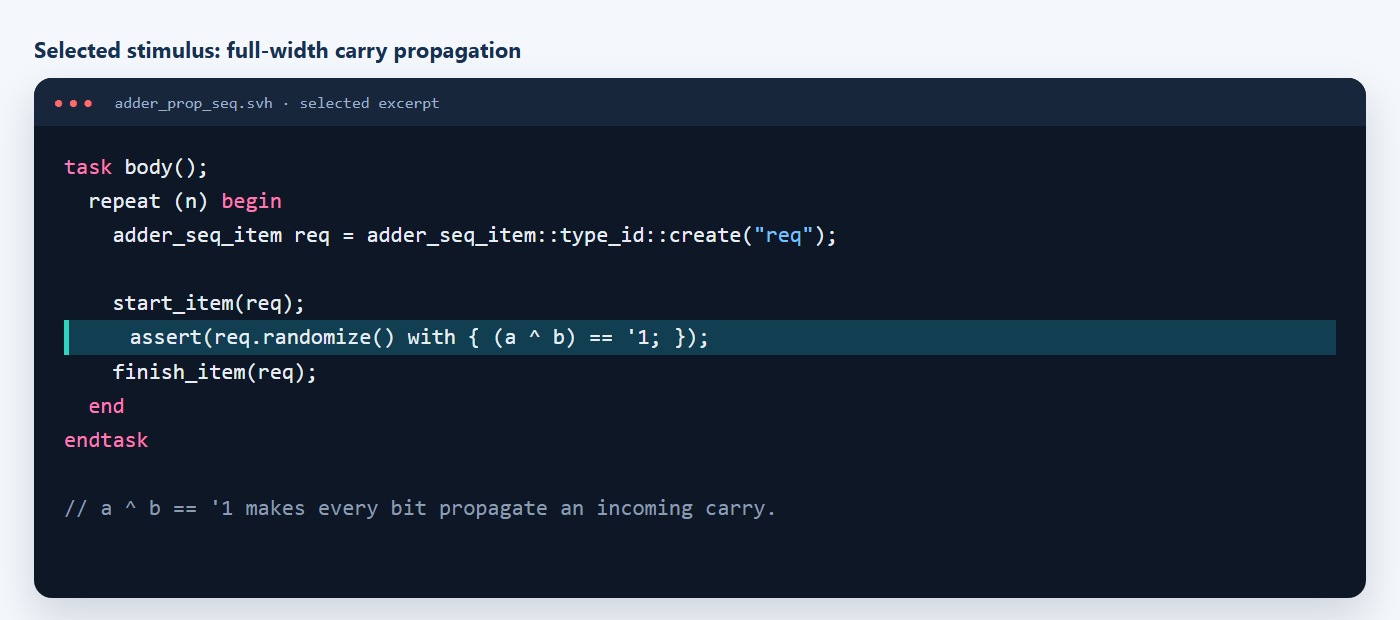
\includegraphics[width=0.96\textwidth]{../p4-adder/figures/full-propagation-sequence.png}
  \caption{Selected full-propagation sequence.}
\end{figure}

\begin{figure}[H]
  \centering
  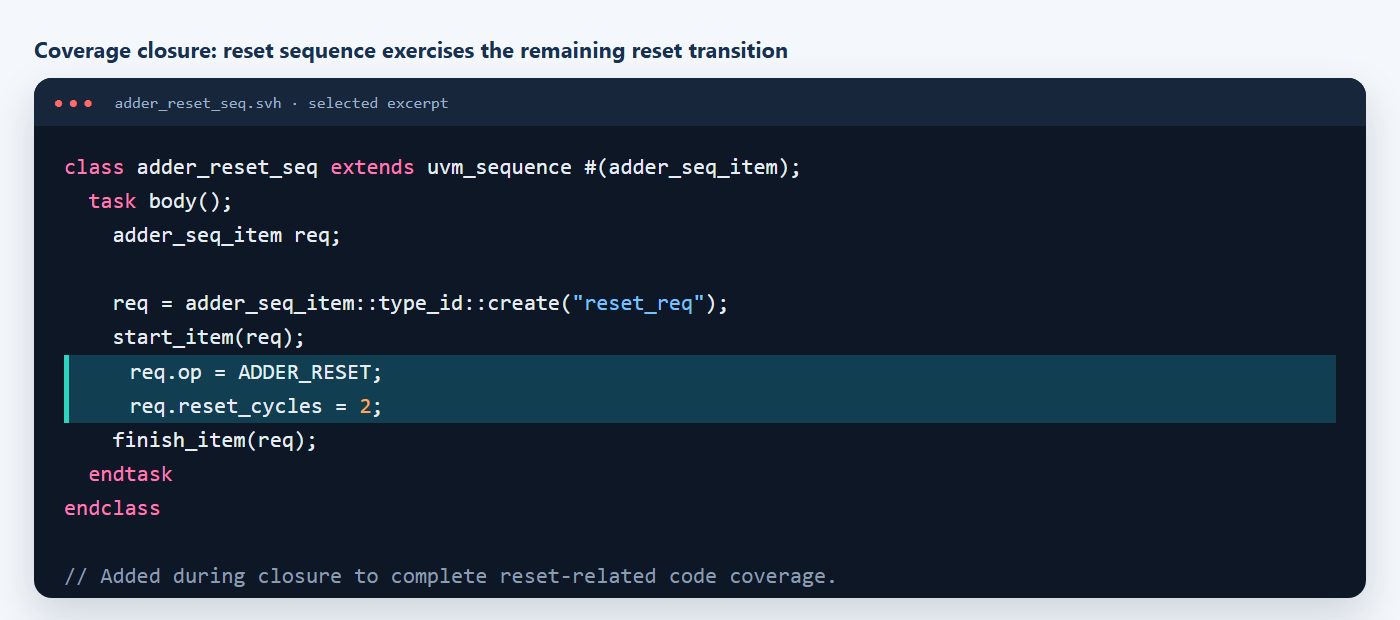
\includegraphics[width=0.96\textwidth]{../p4-adder/figures/reset-sequence.png}
  \caption{Reset sequence added to close reset and registered-wrapper coverage.}
\end{figure}

\subsection{Functional coverage groups}

Operand-value bins alone do not describe whether the carry architecture was exercised. The coverage model instead derives, for every 4-bit block, the group propagate \(p_i\), group generate \(g_i\), carry entering the block, and the ripple condition \(p_i\land c_i\). A covergroup with an explicit sample function is sampled once for every block.

\begin{table}[H]
\centering
\caption{P4 functional coverage model.}
\begin{tabularx}{0.94\textwidth}{@{}p{0.33\textwidth}Y@{}}
\toprule
\textbf{Coverpoint or cross} & \textbf{Verification question} \\
\midrule
Block index & Was every 4-bit carry block sampled? \\
Propagate and generate & Was each block observed in both architectural conditions? \\
Carry ripple & Did a carry actually cross a block boundary? \\
Block by propagate/generate & Were propagate and generate reached at every block position? \\
Block by ripple & Did a carry ripple through every one of the eight blocks? \\
Carry input, carry output, full propagation & Were top-level carry behavior and the critical full-width case exercised? \\
Illegal \((p,g)=(1,1)\) & Did the coverage derivation ever report an impossible state? \\
\bottomrule
\end{tabularx}
\end{table}

\begin{figure}[H]
  \centering
  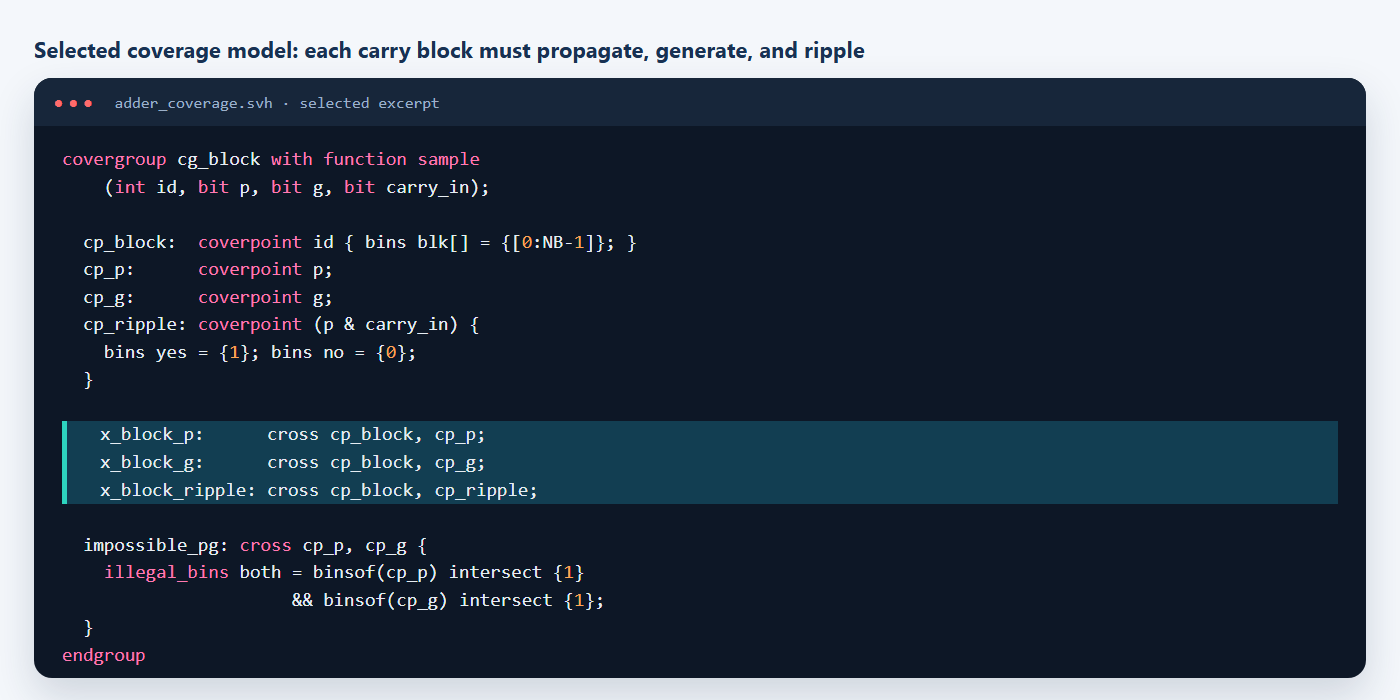
\includegraphics[width=0.99\textwidth]{../p4-adder/figures/coverage-bins.png}
  \caption{Selected P4 coverpoints, per-block crosses, and the impossible-state illegal bin.}
\end{figure}

\subsection{Coverage closure and results}

Coverage closure followed the reports rather than a larger random transaction count. Directed vectors exercised non-masking combinations in the prefix equations. A reset sequence closed the remaining reset-related bins and transitions. The final RTL report records complete functional, statement, branch, expression, toggle, and assertion coverage.

Two testbench issues were also found while closing coverage. Unsigned operand-width types were required for high-value coverage ranges, avoiding signed truncation of values such as \code{32'hF0000000}. The test also needed a drain period before dropping its UVM objection so the final registered transactions could leave the DUT and monitor pipeline.

The same UVM environment was reused against the mapped netlist with back-annotated timing. The functional model again reached 117 of 117 bins. A deliberate fault-injection run also produced scoreboard mismatches and returned to zero errors when the fault was removed, confirming that the checker was capable of rejecting an incorrect result.

\begin{table}[H]
\centering
\caption{P4 verification and synthesis results.}
\begin{tabularx}{0.88\textwidth}{@{}Y>{\raggedleft\arraybackslash}p{0.31\textwidth}@{}}
\toprule
\textbf{Metric} & \textbf{Result} \\
\midrule
Scoreboard & 601 checks, 0 mismatches \\
Functional coverage & 100\% (117/117 bins) \\
Statement coverage & 100\% \\
Branch coverage & 100\% \\
Expression coverage & 100\% \\
Toggle coverage & 100\% \\
Assertion coverage & 100\% (14/14) \\
Filtered overall RTL coverage & 100\% \\
Post-synthesis functional coverage & 100\% (117/117 bins) \\
Post-synthesis filtered coverage & 99.95\% \\
Post-synthesis toggle coverage & 99.86\% (761/762) \\
Clock constraint & 2.00 ns \\
Worst timing slack & 0.01 ns, met \\
\bottomrule
\end{tabularx}
\end{table}

\section{Windowed register-file verification}

\subsection{Verification goal and checklist}

The verification goal is to prove the logical register view, moving window state, and registered read behavior on every clock, including the overflow and underflow boundaries.

\begin{table}[H]
\centering
\caption{Windowed register-file specification checklist.}
\begin{tabularx}{0.97\textwidth}{@{}p{0.28\textwidth}Y@{}}
\toprule
\textbf{Requirement} & \textbf{Acceptance criterion} \\
\midrule
Reset state & Clear the 136-entry array; initialize CWP and SWP to 0, \code{CANSAVE} to 7, \code{CANRESTORE} to 0, and both boundary flags low. \\
Address translation & Map IN, LOCAL, and OUT through CWP with modulo-128 wrap-around; map globals to fixed physical registers 128--135. \\
Window overlap & After \code{CALL}, caller OUT and callee IN resolve to the same eight physical registers. \\
Data timing & Verify both registered read ports, one-cycle latency, read-before-write behavior, and defined idle cycles. \\
Control priority & Verify \code{CALL} over \code{RET} over normal access, and state hold when disabled. \\
Window state & Verify CWP/SWP movement, every save/restore counter value, and single-cycle \code{SPILL}/\code{FILL} pulses. \\
Boundary semantics & Compare overflow and underflow behavior with the expected new-window allocation and identify any mismatch. \\
RAL and netlist reuse & Backdoor-check the eight fixed-map globals and reuse the environment against the mapped netlist. \\
\bottomrule
\end{tabularx}
\end{table}

\subsection{RTL behavior and address mapping}

The design exposes 32 logical 64-bit registers: eight input, eight local, eight output, and eight global registers. Eight windows occupy 128 physical registers, while the global block occupies fixed physical locations 128 through 135. Each window spans 24 physical locations, and a \code{CALL} advances the current window pointer by 16. The caller's output block and the callee's input block therefore share the same eight physical registers.

The window-management state contains the current and saved window pointers (CWP and SWP), plus \code{CANSAVE} and \code{CANRESTORE}. When the available-window pool is exhausted, \code{CALL} raises \code{SPILL}; the reverse boundary raises \code{FILL}.

\begin{figure}[H]
  \centering
  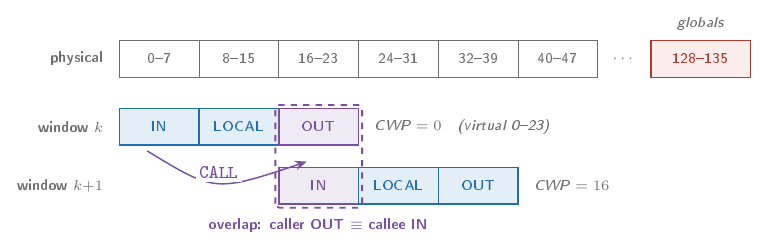
\includegraphics[width=0.98\textwidth]{../windowed-register-file/figures/window-overlap.png}
  \caption{Logical-to-physical mapping and the overlap between adjacent windows.}
\end{figure}

\clearpage
\subsection{UVM environment}

Every clock is meaningful for this DUT, so a sequence item represents one complete cycle: reset, enable, call, return, read/write controls, logical addresses, input data, and the observed registered responses. The driver uses non-blocking item retrieval and drives an explicit idle when no item is pending. This prevents one-shot controls such as \code{CALL}, \code{RET}, and write enable from remaining asserted across an idle cycle.

The monitor uses a one-entry pipeline because reads are registered. It pairs the inputs accepted at cycle \(T\) with the outputs visible at \(T+1\), then broadcasts the complete cycle to the scoreboard. Tests include a drain period before ending so the last pending response is checked.

\begin{figure}[H]
  \centering
  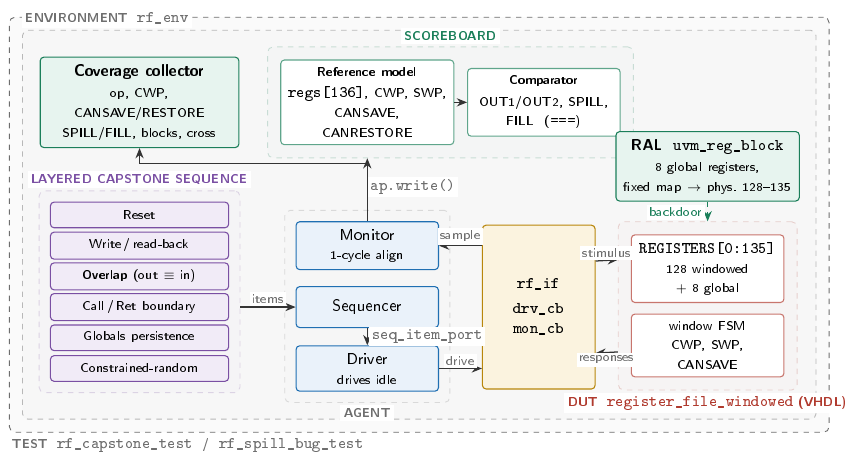
\includegraphics[width=0.99\textwidth]{../windowed-register-file/figures/uvm-environment.png}
  \caption{Windowed register-file UVM environment. The scoreboard contains the stateful reference model and functional coverage.}
\end{figure}

\subsection{Independent cycle-accurate reference model}

The scoreboard contains an independent SystemVerilog model of the complete functional state:

\begin{itemize}
  \item the 136-entry physical register array;
  \item virtual-to-physical translation with wrap-around for the 128 windowed locations and fixed mapping for the eight globals;
  \item CWP, SWP, \code{CANSAVE}, and \code{CANRESTORE};
  \item registered outputs and the \code{SPILL}/\code{FILL} pulse behavior;
  \item read-before-write behavior when the same location is read and written in one cycle;
  \item the priority of \code{CALL}/\code{RET} over an access in the same cycle;
  \item reset behavior, including the fact that the RTL resets the array and state but does not reset the output registers.
\end{itemize}

The model advances once for every monitored cycle and predicts both read ports and both boundary flags. Because the model already owns the reference values of CWP and the counters, those values are passed directly into the coverage group. This avoids a second, potentially inconsistent reconstruction of the internal state.

\subsection{Stimulus and state-space exploration}

The layered capstone sequence combines write/read-back, adjacent-window overlap, repeated calls and returns, global-register persistence, constrained-random traffic, and a coverage-closure sweep. The overlap sequence writes unique values through the caller's output registers, performs a \code{CALL}, then reads the callee's input registers. Any translation error produces shifted or incorrect values.

The call/return sequence deliberately exceeds both boundaries: seven successful allocations are followed by additional calls that must pulse \code{SPILL}, then extra returns reach \code{FILL}. The sweep sequence visits every CWP position and performs idle and access operations at each window before unwinding.

\begin{figure}[H]
  \centering
  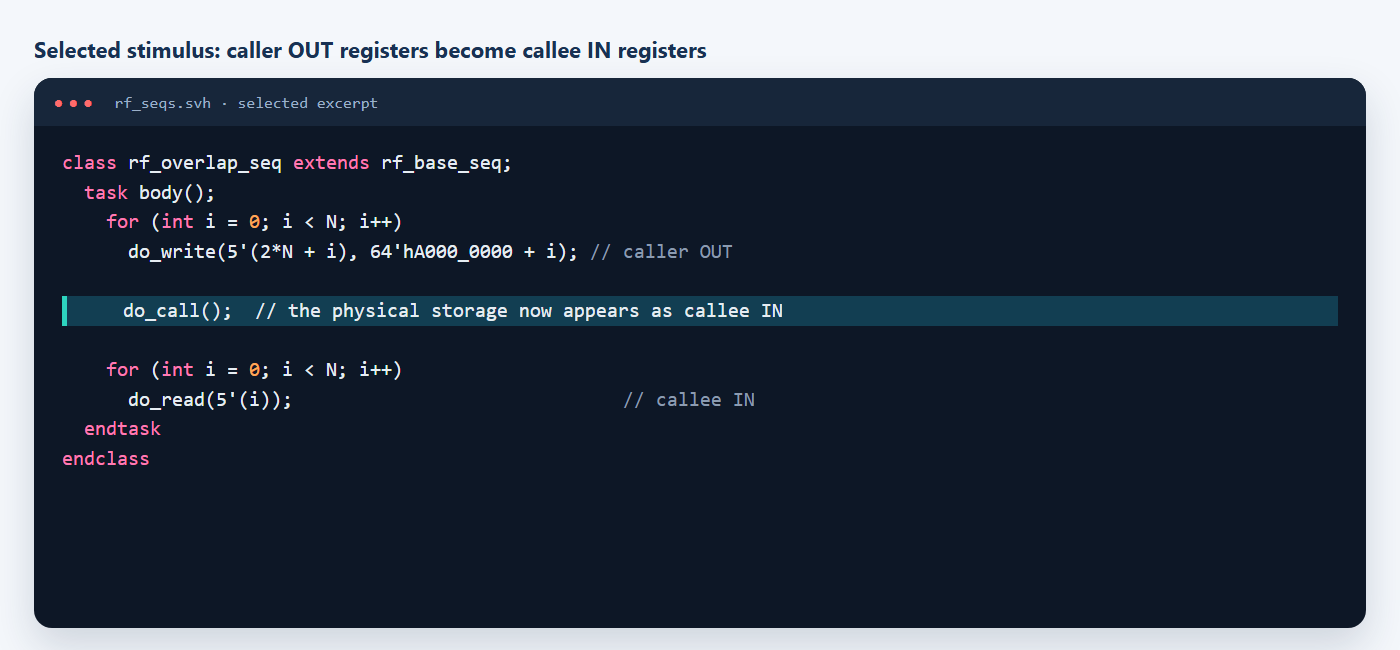
\includegraphics[width=0.97\textwidth]{../windowed-register-file/figures/overlap-sequence.png}
  \caption{Selected adjacent-window overlap sequence.}
\end{figure}

\subsection{Functional coverage of the FSM and counters}

The functional coverage group targets the internal window-management state rather than arbitrary data values. It samples eight coverage quantities:

\begin{table}[H]
\centering
\caption{Register-file functional coverage model.}
\begin{tabularx}{0.94\textwidth}{@{}p{0.30\textwidth}Y@{}}
\toprule
\textbf{Coverpoint or cross} & \textbf{Coverage intent} \\
\midrule
Operation & Reset, call, return, normal access, and idle. \\
CWP & All eight current-window positions: 0, 16, 32, 48, 64, 80, 96, and 112. \\
\code{CANSAVE} & Every occupancy value from 0 through 7. \\
\code{CANRESTORE} & Every occupancy value from 0 through 7. \\
\code{SPILL} and \code{FILL} & Both inactive and asserted values for each boundary event. \\
Addressed block & Input, local, output, global, and no-access cycles. \\
Operation by CWP & Each reachable operation at every reachable window position. \\
\bottomrule
\end{tabularx}
\end{table}

\begin{figure}[H]
  \centering
  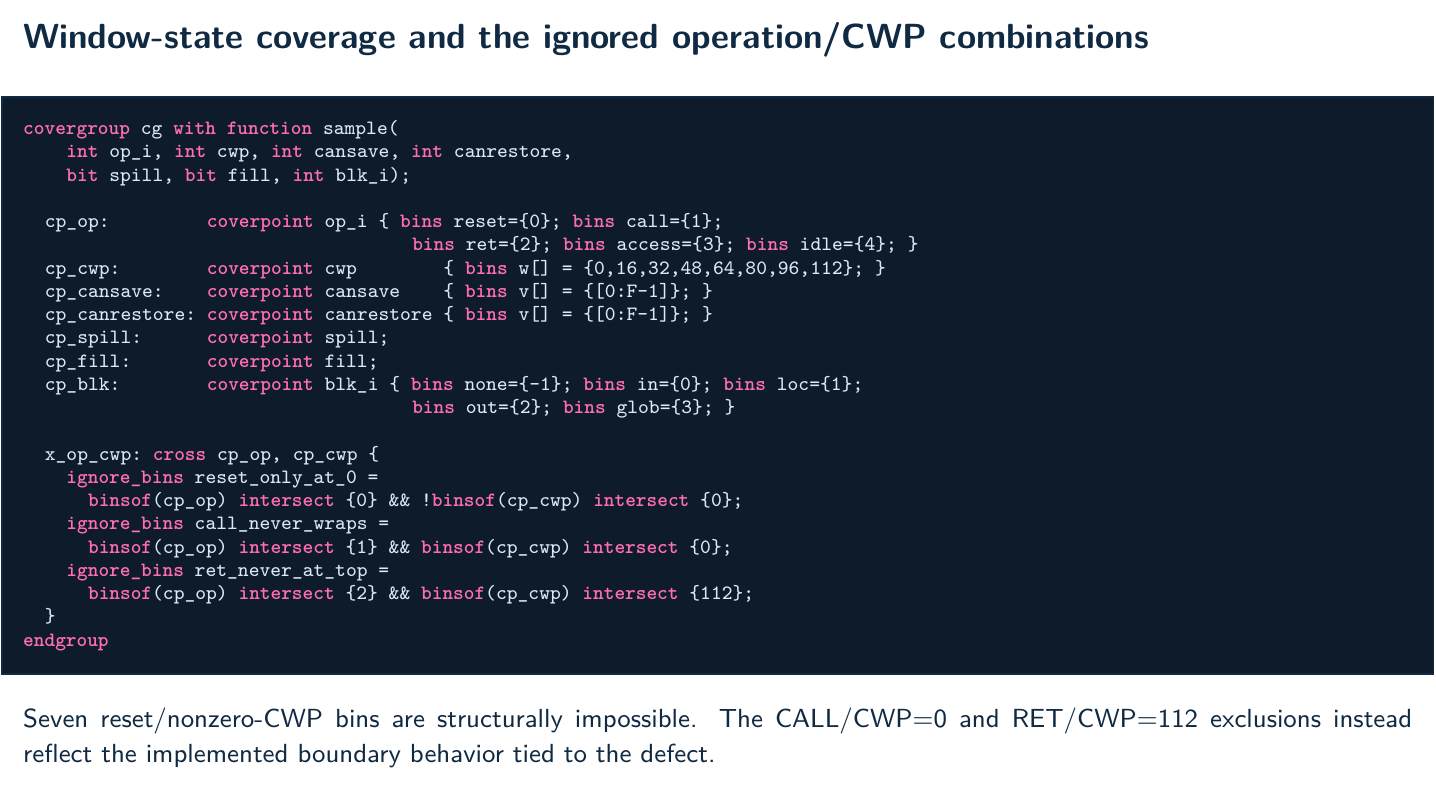
\includegraphics[width=0.99\textwidth]{../windowed-register-file/figures/coverage-bins.png}
  \caption{Selected register-file coverpoints and the operation-by-window cross.}
\end{figure}

The current covergroup contains three \code{ignore\_bins} declarations that remove nine operation-by-CWP combinations from the denominator. Seven are structurally impossible because reset forces CWP to zero. The remaining two are CALL sampled at CWP 0 and RET sampled at CWP 112. Those two are absent under the implemented spill/fill behavior and therefore relate to the boundary defect rather than to an inherent specification constraint. The preserved reports contain only the resulting model and show 69 of 69 bins covered; no pre-exclusion report is available to support a separate ``initial'' percentage. Thus, 69 of 69 describes the reduced functional model. The two RTL statement and branch misses remained visible in code coverage and exposed the same boundary problem.

\subsection{RAL boundary}

UVM RAL assumes a fixed logical address-to-register mapping. The moving window region violates that assumption because the same logical address resolves to a different physical register after \code{CALL} or \code{RET}. The eight global registers do have a fixed mapping, so the RAL block models only those registers.

Each 64-bit global is represented by a \code{uvm\_reg} object with a fixed HDL path to physical registers 128 through 135. The RAL exercise is implemented directly in \code{rf\_ral\_test}, not as a separate UVM sequence class. Its build phase constructs the block and sets the DUT HDL root; its run phase loops over all eight globals, writes each with backdoor \code{poke}, reads it with \code{peek}, and compares the returned value. The windowed data plane remains under the cycle-accurate reference model.

\begin{figure}[H]
  \centering
  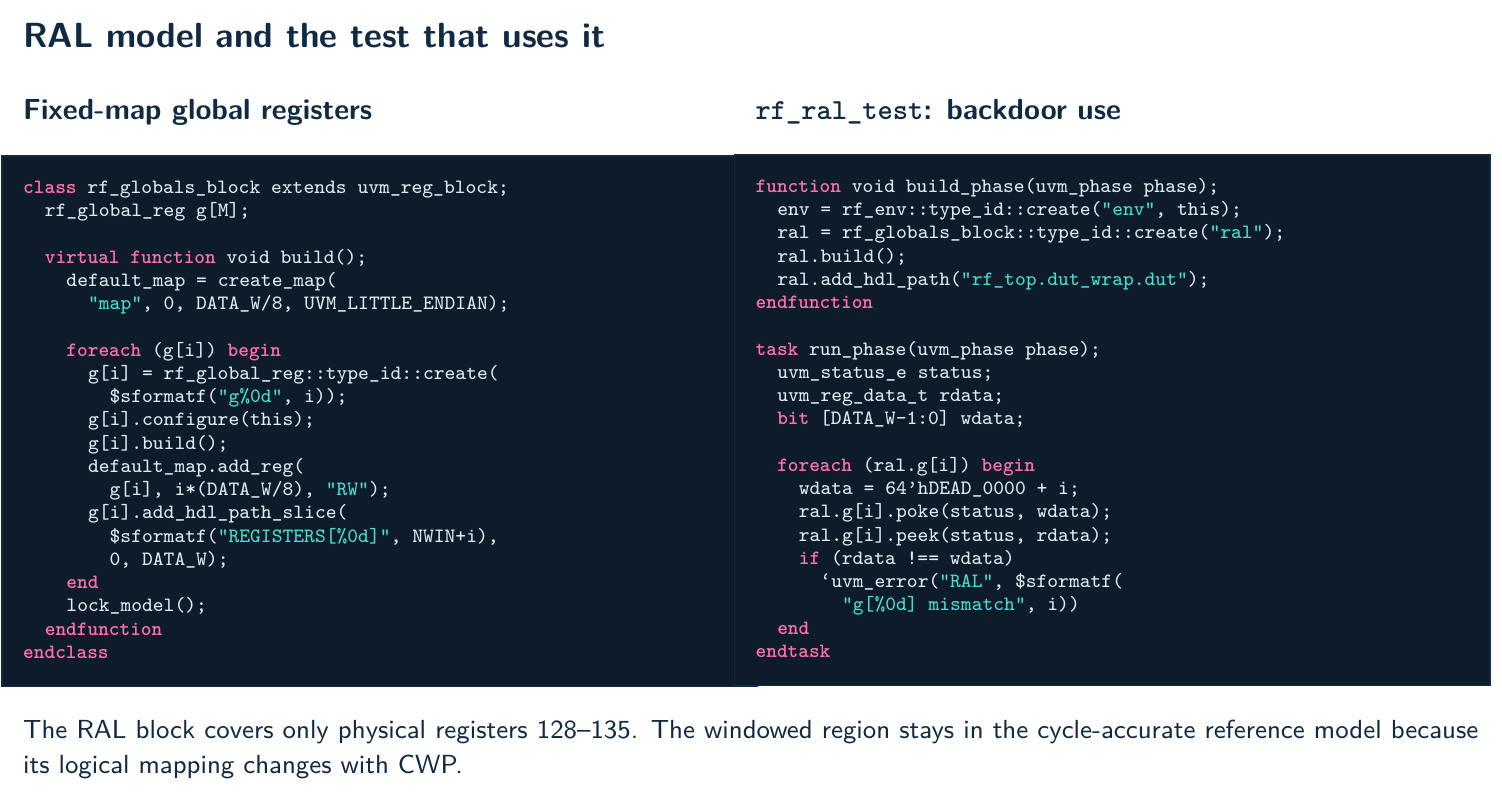
\includegraphics[width=0.99\textwidth]{../windowed-register-file/figures/ral-model-and-test.png}
  \caption{Selected RAL model code and the \code{rf\_ral\_test} backdoor \code{poke}/\code{peek} loop.}
\end{figure}

\subsection{Results and coverage closure}

\begin{table}[H]
\centering
\caption{Windowed register-file verification and synthesis results.}
\begin{tabularx}{0.90\textwidth}{@{}Y>{\raggedleft\arraybackslash}p{0.32\textwidth}@{}}
\toprule
\textbf{Metric} & \textbf{Result} \\
\midrule
Scoreboard & 1,058 checks, 0 mismatches \\
Functional coverage & 100\% (69/69 bins) \\
Statement coverage & 94.73\% (36/38) \\
Branch coverage & 94.59\% (35/37) \\
Toggle coverage & 100\% (438/438) \\
Assertion coverage & 100\% \\
Filtered overall RTL coverage & 97.86\% \\
Post-synthesis functional coverage & 100\% (69/69 bins) \\
Post-synthesis toggle coverage & 38.23\% (23,630/61,808) \\
Clock constraint & 3.00 ns \\
Worst timing slack & 1.36 ns, met \\
\bottomrule
\end{tabularx}
\end{table}

The lower gate-level toggle percentage reflects the size and implementation detail of a 136 by 64 mapped register array. Functional completeness is reported separately through the unchanged covergroup, which again reached 69 of 69 bins.

\subsection{Code coverage exposes the window-overflow defect}

Code coverage revealed the defect. Of 38 RTL statements, the only two not executed were the upward CWP wrap assignment on \code{CALL} and the downward CWP wrap assignment on \code{RET}; the corresponding branches were also the only branch misses. Tracing the control flow from those misses showed why. When \code{CANSAVE} reaches zero, the next \code{CALL} takes the spill path: SWP advances, but CWP, \code{CANSAVE}, and \code{CANRESTORE} remain unchanged. The mirrored condition occurs on fill. The wrap assignments are therefore unreachable, and the next procedure continues to address the caller's current window.

\begin{figure}[H]
  \centering
  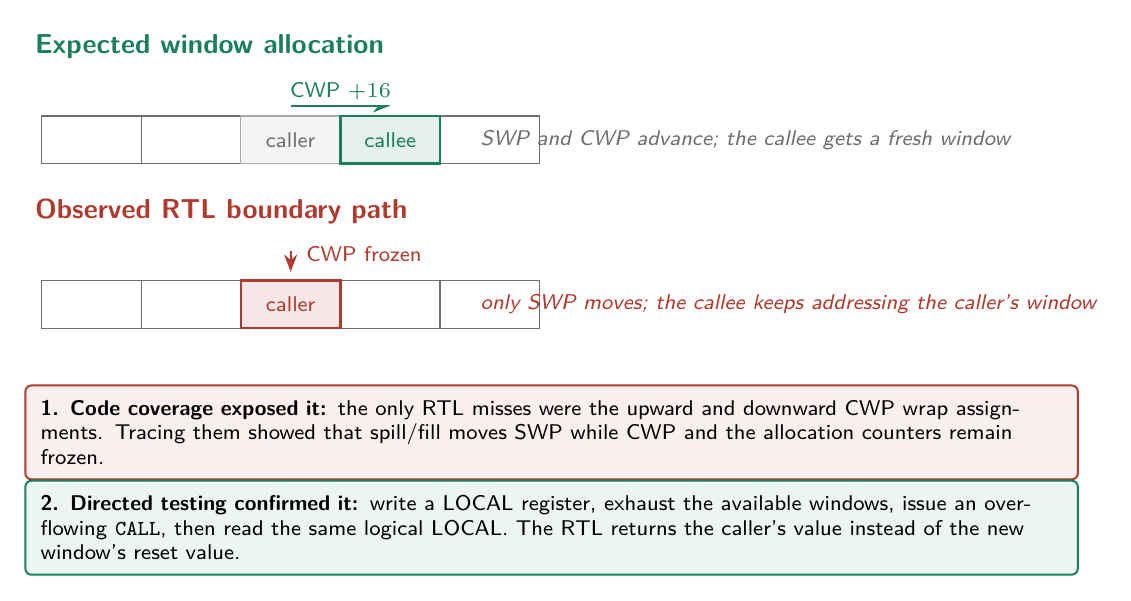
\includegraphics[width=0.98\textwidth]{../windowed-register-file/figures/overflow-finding.png}
  \caption{Code-coverage trigger and directed confirmation of the window-overflow defect.}
\end{figure}

The functional consequence was then confirmed with a specification-oriented reference-model mode and a directed test. In that mode, overflow advances CWP together with SWP and underflow retreats it. The test writes a local register, exhausts the available windows, forces an overflowing \code{CALL}, and reads the same logical local register. Local registers do not overlap, so the newly selected window should contain its reset value. The RTL instead returns the caller's data. The directed failure confirms the design problem first exposed by the code-coverage holes.

\subsection{Post-synthesis findings}

Gate-level verification exposed two additional implementation and testbench details:

\begin{enumerate}
  \item One \code{CANRESTORE} bit could remain unknown after power-up because the mapped design used synchronous-only reset logic. The spill path remained correct while the fill path became unknown. Depositing a defined initial state reproduced physical power-up behavior; an asynchronous reset on the small window-management state would remove the simulation ambiguity.
  \item The first version of the monitored response fields used two-state types. Sampling an unknown gate-level output converted \code{x} to zero before it reached the scoreboard. Changing DUT-sampled fields to four-state \code{logic} preserved the unknown and allowed the strict comparison to report it correctly.
\end{enumerate}

These findings were invisible in the RTL regression and demonstrate why the same environment was reused at the mapped-netlist level.

\section{Conclusion}

The P4 environment verifies a registered arithmetic datapath through aligned transactions, an independent arithmetic model, architecture-aware carry coverage, targeted propagation stimulus, reset closure, and post-synthesis reuse. The register-file environment verifies a stateful mapping problem through one-cycle transactions, an explicit-idle driver, a cycle-accurate model of the physical array and FSM, coverage of the window pointer and counters, directed state-space exploration, and a deliberately limited RAL model for the fixed-map globals.

Both projects reached complete functional coverage at RTL and post synthesis. The separate code-coverage results show different outcomes: complete RTL coverage for the P4 adder, and two unreachable wrap branches in the register file that exposed the overflow defect and led to its directed functional confirmation.

\section{Learning resources}

The UVM methodology and verification techniques used in these projects were studied through:

\begin{itemize}
  \item Ray Salemi, \emph{UVM and SystemVerilog training course}, Siemens.
  \item Ashok B. Mehta, \emph{ASIC/SoC Functional Design Verification: A Comprehensive Guide to Technologies and Methodologies}.
\end{itemize}

\end{document}
